\documentclass{article}
\usepackage{tikz}
\usepackage{pgfplots}
\usepackage{amssymb}
\usepackage[most]{tcolorbox}
\usepackage{gensymb}
\usetikzlibrary{angles,quotes}


\title{\bf{Chapter 12}\\ Variance, Covariance and Correlation}
\date{}

\begin{document}
\maketitle
\section{Variance}
Consider some numbers on 1 Dimension marked as points.\vspace{-5cm}\\
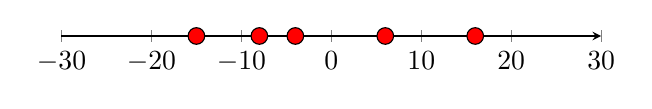
\begin{tikzpicture}
  \begin{axis}[
      xmin=-30, xmax=30,
      axis x line=bottom,% only show the bottom x axis
      hide y axis,
      ymin=0,ymax=5,
      scatter/classes={%
          a={mark=o,draw=black}}
    ]

    \addplot[scatter,only marks,
      mark size = 3pt,
      fill = red,
      scatter src=explicit symbolic]
    table {
        -15 0
        -8 0
        -4 0
        6 0
        16 0
      };
  \end{axis}

\end{tikzpicture}\\
These points are:\\
\begin{tabular}{|c|c|}
  \hline
  {$x$}   & Value \\ \hline
  {$x_1$} & -1    \\ \hline
  {$x_2$} & -8    \\ \hline
  {$x_3$} & -4    \\ \hline
  {$x_4$} & 6     \\ \hline
  {$x_5$} & 16    \\ \hline
\end{tabular}\\\\
Now the mean of this data would be:\\
$$
  \bar{x}=\frac{x_1+x_2+x_3+x_4+x_5}{5}=\frac{-1-8-4+6+16}{5}=\frac{9}{5}=1.8
$$
\\Let's plot this mean on our number line\vspace{-5cm}\\
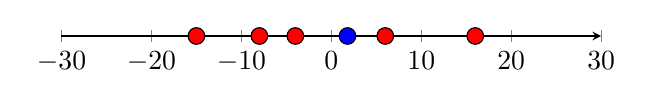
\begin{tikzpicture}
  \begin{axis}[
      xmin=-30, xmax=30,
      axis x line=bottom,% only show the bottom x axis
      hide y axis,
      ymin=0,ymax=5,
      scatter/classes={%
          a={mark=o,draw=black}}
    ]

    % plotting the data points
    \addplot[scatter,only marks,
      mark size = 3pt,
      fill = red,
      scatter src=explicit symbolic]
    table {
        -15 0
        -8 0
        -4 0
        6 0
        16 0
      };
    % Plotting the mean of the data

    \addplot[scatter,only marks,
      mark size = 3pt,
      fill = blue,
      scatter src=explicit symbolic]
    table {
        1.8 0
      };
  \end{axis}

\end{tikzpicture}\\
Here mean is represented using blue color and all the data points are red colored\\\\
Now, what if we need to find how much separated are these points from the mean\\
or, the average distance of all these points from the mean\\
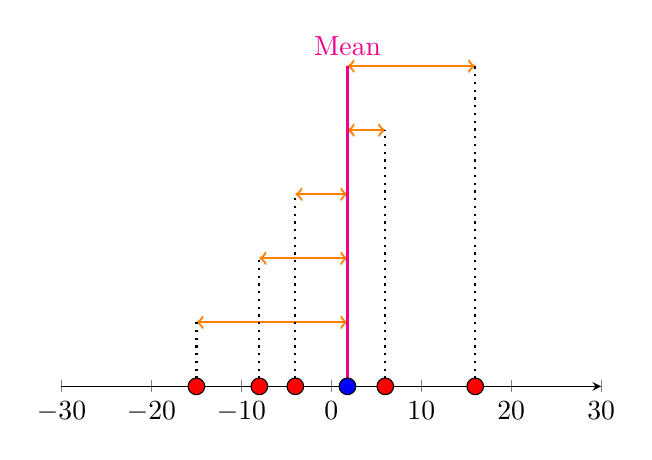
\begin{tikzpicture}
  \begin{axis}[
      xmin=-30, xmax=30,
      axis x line=bottom,% only show the bottom x axis
      hide y axis,
      ymin=-0, ymax=7,
      scatter/classes={%
          a={mark=o,draw=black}}
    ]

    % plotting the data points
    \addplot[scatter,only marks,
      mark size = 3pt,
      fill = red,
      scatter src=explicit symbolic]
    table {
        -15 0
        -8 0
        -4 0
        6 0
        16 0
      };

    % Plotting the mean of the data
    \addplot[scatter,only marks,
      mark size = 3pt,
      fill = blue,
      scatter src=explicit symbolic]
    table {
        1.8 0
      };


    % Drawing lines between mean and data points
    \draw[<->,thick,orange] (axis cs:-15, 1) -- (axis cs:1.8, 1);
    \draw[<->,thick,orange] (axis cs:-8, 2) -- (axis cs:1.8, 2) ;
    \draw[<->,thick,orange] (axis cs:-4, 3) -- (axis cs:1.8, 3) ;
    \draw[<->,thick,orange] (axis cs:6, 4) -- (axis cs:1.8, 4)  ;
    \draw[<->,thick,orange] (axis cs:16, 5) -- (axis cs:1.8, 5) ;

    % drawing vertical lines

    \draw[thick,magenta] (axis cs:1.8, 0)--(axis cs:1.8, 5) node[above,pos=1]{Mean};
    \draw[dotted,thick] (axis cs:-15, 0)--(axis cs:-15, 1) ;
    \draw[dotted,thick] (axis cs:-8, 0)--(axis cs:-8, 2) ;
    \draw[dotted,thick] (axis cs:-4, 0)--(axis cs:-4, 3) ;
    \draw[dotted,thick] (axis cs:6, 0)--(axis cs:6, 4) ;
    \draw[dotted,thick] (axis cs:16, 0)--(axis cs:16, 5) ;


  \end{axis}
\end{tikzpicture}\\


We can do this by calculating each point's distance from the mean and the finding average of all those distances\\
Note that distances can be negative and might result in making the overall average 0, so distances would be squared.\\
$
  D_{x_1,\bar{x}} = (\bar{x}-x_1)^2=(1.5-(-15))^2=272 \\
  D_{x_2,\bar{x}} = (\bar{x}-x_2)^2=(1.5-(-8))^2=90.25 \\
  D_{x_3,\bar{x}} = (\bar{x}-x_3)^2=(1.5-(-4))^2= 30.25\\
  D_{x_4,\bar{x}} = (\bar{x}-x_4)^2=(1.5-6)^2= 20.25\\
  D_{x_5,\bar{x}} = (\bar{x}-x_5)^2=(1.5-16)^2=210.25 \\
$
Now,\\
$
  D_{Average}=\frac{D_{x_1,\bar{x}}+D_{x_2,\bar{x}}+D_{x_3,\bar{x}}+D_{x_4,\bar{x}}+D_{x_5,\bar{x}}+D_{x_6,\bar{x}}}{6}\\\\=\frac{272+90.25+30.25+20.25+210.25}{5}=124.6
$\\\\

This average distance of points with mean is actually called "Variance"\\
Hence, Sample Variance is given by\\
$$
  Var(x)=\frac{\sum_{i=1}^{n}(\bar{x}-x_{i})^2}{1-n}
$$\\
\pagebreak
\section{Covariance}

Now, what if instead of just 1 Dimension there were 2 Dimensions and the data had two parameters x and y?\\\\
For example here are the points:\\\\
\begin{tabular}{|c|c|}
  \hline
  {$x$} & {$y$} \\ \hline
  -15   & -2    \\ \hline
  -8    & 4     \\ \hline
  -4    & -3    \\ \hline
  6     & 3     \\ \hline
  10    & 9     \\ \hline
  16    & 6     \\ \hline
\end{tabular}\\\\

The plot would look like this\\\\
\begin{tikzpicture}
  \begin{axis}[
      xmin=-20, xmax=20,
      ymin=-20,ymax=20,
      % axis x line=bottom,% only show the bottom x axis
      % hide y axis,    
      axis lines=middle,
      xlabel=$x$,
      ylabel=$y$,
      scatter/classes={%
          a={mark=o,draw=black}}
    ]

    \addplot[scatter,only marks,
      mark size = 3pt,
      fill = red,
      scatter src=explicit symbolic]
    table {
        -15 -2
        -8 4
        -4 -3
        6 3
        10 9
        16 6
      };

  \end{axis}

\end{tikzpicture}\\
Let's also plot the mean of x and y\\
$$
  \bar{x}=0.834
$$
$$
  \bar{y}=2.834
$$\\


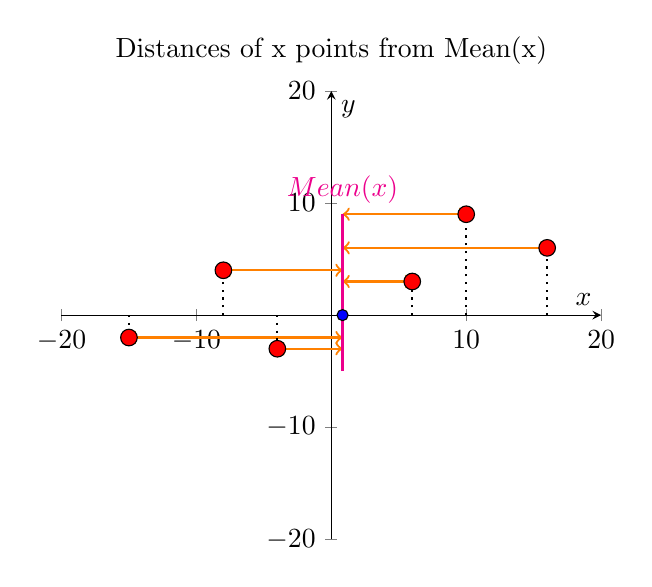
\begin{tikzpicture}
  \begin{axis}[title=Distances of x points from Mean(x),
      xmin=-20, xmax=20,
      ymin=-20,ymax=20,
      % axis x line=bottom,% only show the bottom x axis
      % hide y axis,    
      axis lines=middle,
      xlabel=$x$,
      ylabel=$y$,
      scatter/classes={%
          a={mark=o,draw=black}}
    ]

    \addplot[scatter,only marks,
      mark size = 3pt,
      fill = red,
      scatter src=explicit symbolic]
    table {
        -15 -2
        -8 4
        -4 -3
        6 3
        10 9
        16 6
      };
    \addplot[scatter,only marks,
      mark size =2pt,
      fill = blue,
      scatter src=explicit symbolic]
    table {
        0.834 0
        % 0 2.834
      };

    % Drawing lines between mean and data points for x axis
    \draw[<->,thick,orange] (axis cs:-15, -2) -- (axis cs:0.834,-2);
    \draw[<->,thick,orange] (axis cs:-8, 4) -- (axis cs:0.834, 4) ;
    \draw[<->,thick,orange] (axis cs:-4, -3) -- (axis cs:0.834,-3) ;
    \draw[<->,thick,orange] (axis cs:6, 3) -- (axis cs:0.834, 3)  ;
    \draw[<->,thick,orange] (axis cs:10, 9) -- (axis cs:0.834, 9) ;
    \draw[<->,thick,orange] (axis cs:16, 6) -- (axis cs:0.834, 6) ;

    % drawing vertical lines

    \draw[thick,magenta] (axis cs:0.834, -5)--(axis cs:0.834, 9) node[above,pos=1]{$Mean(x)$};
    \draw[dotted,thick] (axis cs:-15, 0)--(axis cs:-15, -2) ;
    \draw[dotted,thick] (axis cs:-8, 0)--(axis cs:-8, 4) ;
    \draw[dotted,thick] (axis cs:-4, 0)--(axis cs:-4,-3) ;
    \draw[dotted,thick] (axis cs:6, 0)--(axis cs:6, 3) ;
    \draw[dotted,thick] (axis cs:10, 0)--(axis cs:10, 9) ;
    \draw[dotted,thick] (axis cs:16, 0)--(axis cs:16, 6) ;
  \end{axis}

\end{tikzpicture}\\\\
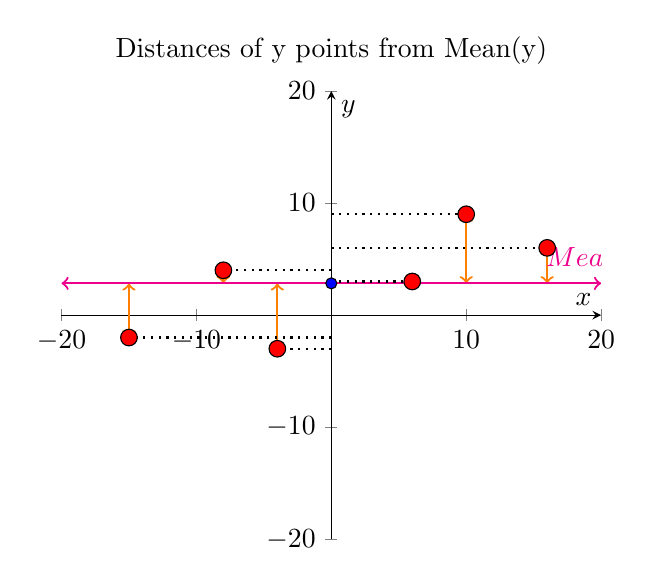
\begin{tikzpicture}
  \begin{axis}[title=Distances of y points from Mean(y),
      xmin=-20, xmax=20,
      ymin=-20,ymax=20,
      % axis x line=bottom,% only show the bottom x axis
      % hide x axis,    
      axis lines=middle,
      xlabel=$x$,
      ylabel=$y$,
      scatter/classes={%
          a={mark=o,draw=black}}
    ]

    \addplot[scatter,only marks,
      mark size = 3pt,
      fill = red,
      scatter src=explicit symbolic]
    table {
        -15 -2
        -8 4
        -4 -3
        6 3
        10 9
        16 6
      };
    \addplot[scatter,only marks,
      mark size =2pt,
      fill = blue,
      scatter src=explicit symbolic]
    table {
        % 1 0
        0 2.834
      };

    % Drawing lines between mean and data points for y axis
    \draw[<->,thick,orange] (axis cs:-15, -2) -- (axis cs:-15,2.834);
    \draw[<->,thick,orange] (axis cs:-8, 4) -- (axis cs:-8,2.834);
    \draw[<->,thick,orange] (axis cs:-4, -3) -- (axis cs:-4,2.834);
    \draw[<->,thick,orange] (axis cs:6, 3) -- (axis cs:6,2.834);
    \draw[<->,thick,orange] (axis cs:10, 9) -- (axis cs:10,2.834);
    \draw[<->,thick,orange] (axis cs:16, 6) -- (axis cs:16,2.834);


    % drawing vertical lines

    \draw[<->,thick,magenta] (axis cs:-20, 2.834)--(axis cs:20, 2.834) node[above,pos=1]{$Mean(y)$};
    \draw[dotted,thick] (axis cs:0, -2)--(axis cs:-15, -2) ;
    \draw[dotted,thick] (axis cs:0, 4)--(axis cs:-8, 4) ;
    \draw[dotted,thick] (axis cs:0, -3)--(axis cs:-4, -3) ;
    \draw[dotted,thick] (axis cs:0, 3)--(axis cs:6, 3) ;
    \draw[dotted,thick] (axis cs:0, 9)--(axis cs:10, 9) ;
    \draw[dotted,thick] (axis cs:0, 6)--(axis cs:16, 6) ;


  \end{axis}

\end{tikzpicture}

Here we can calculate\\\\
Variance along x direction\\ $Var(x)=\frac{\sum_{i=1}^{n}(\bar{x}-x_{i})^2}{1-n}\\=\frac{(-15-0.834)^2+(-8-0.834)^2+(-4-0.834)^2+(6-0.834)^2+(10-0.834)^2+(16-0.834)^2}{5}=138.5666672$\\\\
Variance along y direction\\ $Var(y)=\frac{\sum_{i=1}^{n}(\bar{y}-y_{i})^2}{1-n}\\=\frac{(-2-2.834)^2+(4-2.834)^2+(-3-2.834)^2+(3-2.834)^2+(9-2.834)^2+(6-2.834)^2}{5}=21.3666672$\\\\

And it's really evident from the plot that values of x are more spread from mean than y\\
and thus $Var(x)>Var(y)$\\\\
The main observation here is that,\\
If we change the signs of x values, the plot flips along vertical axis\\\\

\begin{tabular}{|c|c|}
  \hline
  {$x$} & {$y$} \\ \hline
  -15   & -2    \\ \hline
  -8    & 4     \\ \hline
  -4    & -3    \\ \hline
  6     & 3     \\ \hline
  10    & 9     \\ \hline
  16    & 6     \\ \hline
\end{tabular}
$\mathbf{\Longrightarrow}$ \begin{tabular}{|c|c|}
  \hline
  {$x$} & {$y$} \\ \hline
  15    & -2    \\ \hline
  8     & 4     \\ \hline
  4     & -3    \\ \hline
  -6    & 3     \\ \hline
  -10   & 9     \\ \hline
  -16   & 6     \\ \hline
\end{tabular}\\\\\\
\begin{tikzpicture}[baseline=(current bounding box.center)]
  \begin{axis}[
      xmin=-20, xmax=20,
      ymin=-20,ymax=20,
      % axis x line=bottom,% only show the bottom x axis
      % hide y axis,    
      axis lines=middle,
      xlabel=$x$,
      ylabel=$y$,
      scatter/classes={%
          a={mark=o,draw=black}}
    ]

    \addplot[scatter,only marks,
      mark size = 3pt,
      fill = red,
      scatter src=explicit symbolic]
    table {
        -15 -2
        -8 4
        -4 -3
        6 3
        10 9
        16 6
      };

  \end{axis}

\end{tikzpicture}$\mathbf{\Longrightarrow}$\begin{tikzpicture}[baseline=(current bounding box.center)]
  \begin{axis}[
      xmin=-20, xmax=20,
      ymin=-20,ymax=20,
      % axis x line=bottom,% only show the bottom x axis
      % hide y axis,    
      axis lines=middle,
      xlabel=$x$,
      ylabel=$y$,
      scatter/classes={%
          a={mark=o,draw=black}}
    ]

    \addplot[scatter,only marks,
      mark size = 3pt,
      fill = red,
      scatter src=explicit symbolic]
    table {
        15 -2
        8 4
        4 -3
        -6 3
        -10 9
        -16 6
      };

  \end{axis}

\end{tikzpicture}\\\\
But still, the values of $Var(x)$ and $Var(y)$ remains the same as before
$$Var(x)=138.5666672$$
$$Var(y)=21.3666672$$\\\\

We need some other metric too....\\
\pagebreak
$$
  Covariance(x,y)=Cov(x,y)=\frac{1}{n-1}*\sum_{i=1}^{n}(x_i-\bar{x})(y_i-\bar{y})
$$
Ok,but what does $(x_i-\bar{x})(y_i-\bar{y})$ means?\\
\begin{tabular}{|c|c|c|c|c|}
  \hline
  {$x$} & {$y$} & {$(x-\bar{x})$}   & {$(y-\bar{y})$} & {$(x-\bar{x})(y-\bar{y})$}   \\ \hline
  -15   & -2    & -15-0.834=-15.834 & -2-2.834=-4.834 & -15.834 * -4.834 = 76.541556 \\ \hline
  -8    & 4     & -8-0.834=-8.834   & 4-2.834=1.166   & -8.834 * 1.166 = -10.300444  \\ \hline
  -4    & -3    & -4-0.834=-4.834   & -3-2.834=-5.834 & -4.834  * -5.834 = 28.201556 \\ \hline
  6     & 3     & 6-0.834=5.166     & 3-2.834=0.166   & 5.166 * 0.166 = 0.857556     \\ \hline
  10    & 9     & 10-0.834=9.166    & 9-2.834=6.166   & 9.166 * 6.166 = 56.517556    \\ \hline
  16    & 6     & 16-0.834=15.166   & 6-2.834=3.166   & 15.166 * 3.166 = 48.015556   \\ \hline
\end{tabular}\\\\\\
Let's plot this for 1st point\\\\
\begin{tikzpicture}
  \begin{axis}[
      width=10cm, % Set the width of the plot
      height=10cm, % Set the height of the plot
      xmin=-20, xmax=20,
      ymin=-20,ymax=20,
      % axis x line=bottom,% only show the bottom x axis
      % hide y axis,    
      axis lines=middle,
      xlabel=$x$,
      ylabel=$y$,
      scatter/classes={%
          a={mark=o,draw=black}}
    ]

    \addplot[scatter,only marks,
      mark size = 3pt,
      fill = red,
      scatter src=explicit symbolic]
    table {
        -15 -2
      };

    \addplot[scatter,only marks,
      mark size = 3pt,
      fill = blue,
      scatter src=explicit symbolic]
    table {
        0.834 0
        0 2.834
      };

    \draw[-|,thick,violet] (axis cs:-15, -2) -- (axis cs:0.834,-2) node[midway,below]{$x_1-\bar{x}$};
    \draw[-|,thick,violet] (axis cs:-15, -2) -- (axis cs:-15,2.834) node[midway,pos=1,above]{$y_1-\bar{y}$};
    % \draw[<->,thick,orange] (axis cs:-8, 4) -- (axis cs:-8,2.834);
    % \draw[<->,thick,orange] (axis cs:-4, -3) -- (axis cs:-4,2.834);
    % \draw[<->,thick,orange] (axis cs:6, 3) -- (axis cs:6,2.834);
    % \draw[<->,thick,orange] (axis cs:10, 9) -- (axis cs:10,2.834);
    % \draw[<->,thick,orange] (axis cs:16, 6) -- (axis cs:16,2.834);

  \end{axis}

\end{tikzpicture}\\\\
\begin{tcolorbox}[colback=pink!5!white,colframe=purple!75!black]
  Red color: Point 1
  \tcblower
  Blue color: Means of x and y
\end{tcolorbox}
Here, we plotted $(x_1-\bar{x}) and (y_1-\bar{y})$, and it's looking really intuitive that $(x_1-\bar{x})(y_1-\bar{y})$ is just the area within that rectangle..\\\\
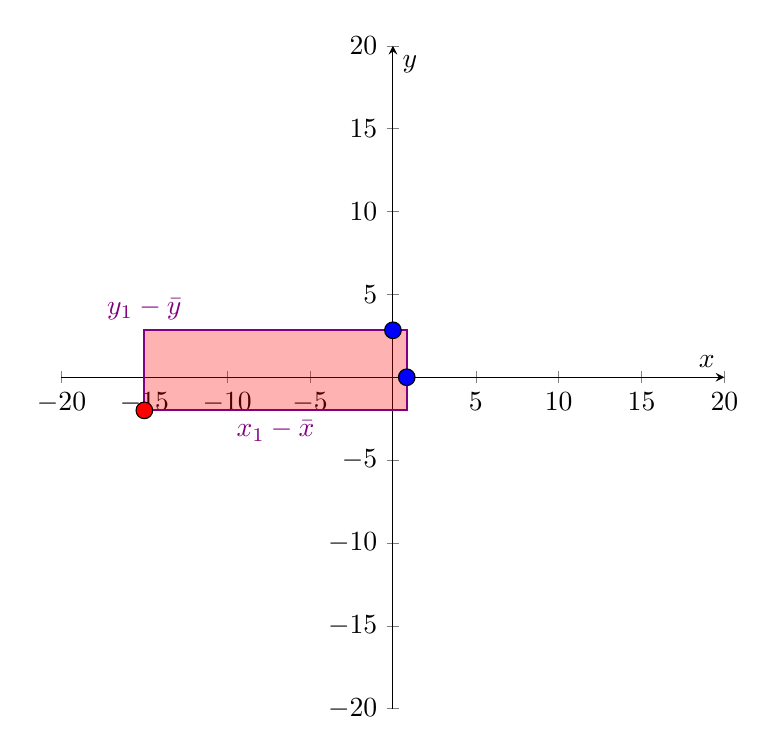
\begin{tikzpicture}
  \begin{axis}[
      width=10cm, % Set the width of the plot
      height=10cm, % Set the height of the plot
      xmin=-20, xmax=20,
      ymin=-20,ymax=20,
      % axis x line=bottom,% only show the bottom x axis
      % hide y axis,    
      axis lines=middle,
      xlabel=$x$,
      ylabel=$y$,
      scatter/classes={%
          a={mark=o,draw=black}}
    ]

    \addplot[scatter,only marks,
      mark size = 3pt,
      fill = red,
      scatter src=explicit symbolic]
    table {
        -15 -2
      };

    \addplot[scatter,only marks,
      mark size = 3pt,
      fill = blue,
      scatter src=explicit symbolic]
    table {
        0.834 0
        0 2.834
      };

    \draw[-,thick,violet] (axis cs:-15, -2) -- (axis cs:0.834,-2) node[midway,below]{$x_1-\bar{x}$};
    \draw[-,thick,violet] (axis cs:0.834,-2) -- (axis cs:0.834,2.834);
    \draw[-,thick,violet] (axis cs:0.834,2.834) -- (axis cs:-15,2.834);
    \draw[-,thick,violet] (axis cs:-15, -2) -- (axis cs:-15,2.834) node[midway,pos=1,above]{$y_1-\bar{y}$};
    \draw[thick,violet,fill=red,fill opacity=0.3] (axis cs:-15, -2) rectangle (axis cs:0.834,2.834);

  \end{axis}

\end{tikzpicture}\\\\
Let's draw this for all points\\
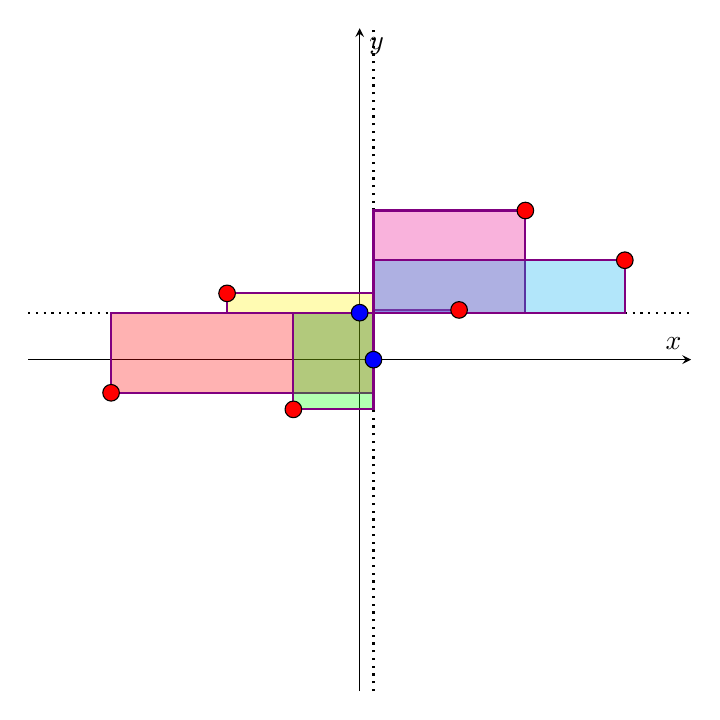
\begin{tikzpicture}
  \begin{axis}[
      ticks=none,
      width=10cm, % Set the width of the plot
      height=10cm, % Set the height of the plot
      xmin=-20, xmax=20,
      ymin=-20,ymax=20,
      % axis x line=bottom,% only show the bottom x axis
      % hide y axis,    
      axis lines=middle,
      xlabel=$x$,
      ylabel=$y$,
      scatter/classes={%
          a={mark=o,draw=black}}
    ]

    \addplot[scatter,only marks,
      mark size = 3pt,
      fill = red,
      scatter src=explicit symbolic]
    table {
        -15 -2
        -8 4
        -4 -3
        6 3
        10 9
        16 6
      };

    \addplot[scatter,only marks,
      mark size = 3pt,
      fill = blue,
      scatter src=explicit symbolic]
    table {
        0.834 0
        0 2.834
      };

    \draw[dotted,thick] (axis cs:0.834,-20)--(axis cs:0.834,20);
    \draw[dotted,thick] (axis cs:-20,2.834)--(axis cs:20,2.834);


    \draw[thick,violet,fill=red,fill opacity=0.3] (axis cs:-15, -2) rectangle (axis cs:0.834,2.834);

    \draw[thick,violet,fill=yellow,fill opacity=0.3] (axis cs:-8, 4) rectangle (axis cs:0.834,2.834);

    \draw[thick,violet,fill=green,fill opacity=0.3] (axis cs:-4, -3) rectangle (axis cs:0.834,2.834);

    \draw[thick,violet,fill=blue,fill opacity=0.3] (axis cs:6, 3) rectangle (axis cs:0.834,2.834);

    \draw[thick,violet,fill=magenta,fill opacity=0.3] (axis cs:10, 9) rectangle (axis cs:0.834,2.834);

    \draw[thick,violet,fill=cyan,fill opacity=0.3] (axis cs:16, 6) rectangle (axis cs:0.834,2.834);

  \end{axis}

\end{tikzpicture}\\\\
\vspace{-5cm}
Now, we need to take signed sum of these areas,\\\\
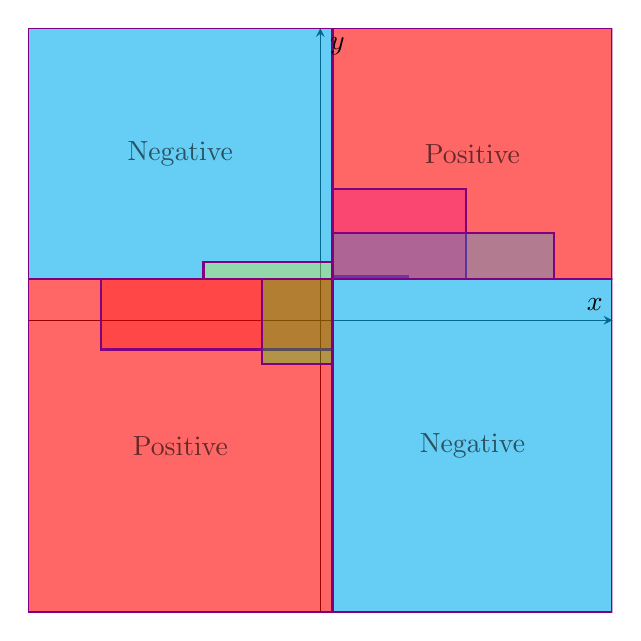
\begin{tikzpicture}
  \begin{axis}[
      ticks=none,
      width=9cm, % Set the width of the plot
      height=9cm, % Set the height of the plot
      xmin=-20, xmax=20,
      ymin=-20,ymax=20,
      % axis x line=bottom,% only show the bottom x axis
      % hide y axis,    
      axis lines=middle,
      xlabel=$x$,
      ylabel=$y$,
      scatter/classes={%
          a={mark=o,draw=black}}
    ]


    \draw[dotted,thick] (axis cs:0.834,-20)--(axis cs:0.834,20);
    \draw[dotted,thick] (axis cs:-20,2.834)--(axis cs:20,2.834);


    \draw[thick,violet,fill=red,fill opacity=0.6] (axis cs:-20, -20) rectangle (axis cs:0.834,2.834) node[midway,thick,black] {Positive};

    \draw[thick,violet,fill=cyan,fill opacity=0.6] (axis cs:-20, 20) rectangle (axis cs:0.834,2.834) node[midway,thick,black] {Negative};

    \draw[thick,violet,fill=red,fill opacity=0.6] (axis cs:20, 20) rectangle (axis cs:0.834,2.834) node[midway,thick,black] {Positive};

    \draw[thick,violet,fill=cyan,fill opacity=0.6] (axis cs:20, -20) rectangle (axis cs:0.834,2.834) node[midway,thick,black] {Negative};

    \draw[thick,violet,fill=red,fill opacity=0.3] (axis cs:-15, -2) rectangle (axis cs:0.834,2.834);

    \draw[thick,violet,fill=yellow,fill opacity=0.3] (axis cs:-8, 4) rectangle (axis cs:0.834,2.834);

    \draw[thick,violet,fill=green,fill opacity=0.3] (axis cs:-4, -3) rectangle (axis cs:0.834,2.834);

    \draw[thick,violet,fill=blue,fill opacity=0.3] (axis cs:6, 3) rectangle (axis cs:0.834,2.834);

    \draw[thick,violet,fill=magenta,fill opacity=0.3] (axis cs:10, 9) rectangle (axis cs:0.834,2.834);

    \draw[thick,violet,fill=cyan,fill opacity=0.3] (axis cs:16, 6) rectangle (axis cs:0.834,2.834);

  \end{axis}

\end{tikzpicture}\\

that would be
$$
  Signed\ Sum\ Of\ Areas=\sum_{i=1}^{n}(x_i-\bar{x})(y_i-\bar{y})
$$
after that we just need to find average value of these signed areas
$$
  \therefore Average\ Signed\ Sum=\frac{Signed\ Sum\ Of\ Areas}{n-1}=\frac{\sum_{i=1}^{n}(x_i-\bar{x})(y_i-\bar{y})}{n};
$$
But what does this average signed sum of areas tell us?\\
A lot actually,
\begin{itemize}

  \item if this value is positive, this means the slope of the best fit line would be positive, this means value of y increases with increase in x.
  \item if this value is negative, this means the slope of the best fit line would be negative, this means value of y decreases with increase in x.
  \item if this value is large, this means there is on an average a large separation between values of x and y with their means, i.e., values are more spread from mean.
  \item if this value is small, this means there is on an average very less sepration between values of x and y with their means, i.e, values are less spread from mean.
  \item if this value is 0, slope is 0, and no linear relationship exist between $x$ and $y$.
\end{itemize}
and since, this value is giving us an idea about how 2 values x and y are varying\\
that is why it is called "Covariance(x,y)"\\
Hence, the formula
$$
  Covariance(x,y)=Cov(x,y)=\frac{1}{n-1}*\sum_{i=1}^{n}(x_i-\bar{x})(y_i-\bar{y})
$$

So, this formula tells about relation between 2 variables but still doesnt tell us anything about the "Strength" of this relation.
Let us now find that strength.\\
\section{Correlation}
If we consider the two variables $x$ and $y$ as vectors.\\
$$
  \vec{x}=\begin{bmatrix}
    x_1    \\
    x_2    \\
    x_3    \\
    \vdots \\
    x_n    \\
  \end{bmatrix} \in \mathbb{R}^n
$$
$$
  \vec{y}=\begin{bmatrix}
    y_1    \\
    y_2    \\
    y_3    \\
    \vdots \\
    y_n    \\
  \end{bmatrix}\\ \in \mathbb{R}^n
$$
but representing an "n" dimensional vector on a 2D plot is not possible, so let's just consider $n=2$\\
$
  \therefore
$
$$
  \vec{x}=\begin{bmatrix}
    x_1 \\
    x_2 \\
  \end{bmatrix} \in \mathbb{R}^2
$$
$$
  \vec{y}=\begin{bmatrix}
    y_1 \\
    y_2 \\
  \end{bmatrix}\\ \in \mathbb{R}^2
$$
\pagebreak
\\
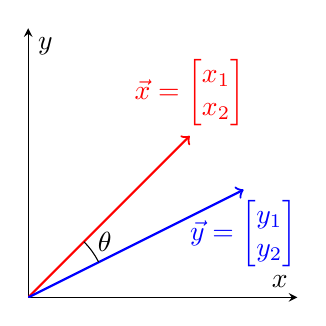
\begin{tikzpicture}
  \begin{axis}[
      ticks=none,
      width=5cm, % Set the width of the plot
      height=5cm, % Set the height of the plot
      xmin=0, xmax=5,
      ymin=0,ymax=5,
      % axis x line=bottom,% only show the bottom x axis
      % hide y axis,    
      axis lines=middle,
      xlabel=$x$,
      ylabel=$y$,
      scatter/classes={%
          a={mark=o,draw=black}}
    ]

    \addplot[fill=black] coordinates {(0,0)} coordinate (O) node[anchor=north] {$O$};
    \addplot[->,thick,red] coordinates {(0,0) (3,3)} coordinate (a) node[pos=1,above]{$\vec{x}=\begin{bmatrix}
            x_1 \\
            x_2 \\
          \end{bmatrix}$};
    \addplot[->,thick,blue] coordinates {(0,0) (4,2)} coordinate (b) node[pos=1,below]{$\vec{y}=\begin{bmatrix}
            y_1 \\
            y_2 \\
          \end{bmatrix}$};
    \pic [draw, angle eccentricity=1.2, angle radius=1cm,"$\theta$"] {angle=b--O--a};
  \end{axis}

\end{tikzpicture}\\
Here $\theta$ is the angle between $\vec{x}$ and $vec{y}$\\\\
Now, we can find how 'related' or 'close' are 2 vectors, using the dot product.

$$
  cos(\theta)=\frac{\vec{x}\cdot\vec{y}}{||\vec{x}||.||\vec{y}||}=\frac{<\vec{x},\vec{y}>}{\sqrt{<x,x>}.\sqrt{<y,y>}}=\frac{x_1.y_1+x_2.y_2}{\sqrt{x_1^2+x_2^2}.\sqrt{y_1^2+y_2^2}}
$$

for n dimensional vectors
$$
  cos(\theta)=\frac{\vec{x}\cdot\vec{y}}{||\vec{x}||.||\vec{y}||}=\frac{<\vec{x},\vec{y}>}{\sqrt{<x,x>}.\sqrt{<y,y>}}=\frac{x_1.y_1+x_2.y_2+\dots+x_n.y_n}{\sqrt{x_1^2+x_2^2+\dots+x_n^2}.\sqrt{y_1^2+y_2^2+\dots+y_n^2}}
$$
$$
  cos(\theta)=\frac{\sum_{i=1}^{n}(x_i.y_i)}{\sqrt{\sum_{i=1}^{n}(x_i^2)}.\sqrt{\sum_{i=1}^{n}(y_i^2)}}
$$
\\
Now consider, this table of values of x and y

\begin{tabular}{|l|l|}
  \hline
  \textbf{x} & \textbf{y} \\
  \hline
  1          & 200        \\
  2          & 240        \\
  2.5        & 340        \\
  3          & 500        \\
  4.5        & 620        \\
  \hline
\end{tabular}
\\
We don't actually need a relation between these 2 variables, we actually want relation between the spreading of these 2 variables from their mean.\\
\pagebreak

We can calculate how far are each points on x and y from their mean $\bar{x}$ and $\bar{y}$\\
\begin{tabular}{|l|l|l|l|}
  \hline
  \textbf{x} & \textbf{y} & \textbf{$x-\bar{x}$} & \textbf{$y-\bar{y}$} \\
  \hline
  1          & 200        & -1.6                 & -180                 \\
  2          & 240        & -0.6                 & -140                 \\
  2.5        & 340        & -0.1                 & -40                  \\
  3          & 500        & 0.4                  & 220                  \\
  4.5        & 620        & 1.9                  & 340                  \\
  \hline
\end{tabular}
\\\\
So, we would consider $\vec{x-\bar{x}}$ and $\vec{y-\bar{y}}$ as the vectors we need to find relation between.
$$
  \vec{x^*}=\vec{x-\bar{x}}=\begin{bmatrix}
    -1.6 \\
    -0.6 \\
    -0.1 \\
    0.4  \\
    1.9  \\
  \end{bmatrix}
$$
$$
  \vec{y^*}=\vec{y-\bar{y}}=\begin{bmatrix}
    -180 \\
    -140 \\
    -40  \\
    220  \\
    340  \\
  \end{bmatrix}
$$

$\therefore$
$$
  cos(\theta)=\frac{\sum_{i=1}^{n}(x_i^*.y_i^*)}{\sqrt{\sum_{i=1}^{n}(x_i^{*2})}.\sqrt{\sum_{i=1}^{n}(y_i^{*2})}}=\frac{\sum_{i=1}^{n}(x_i-\bar{x}).(y_i-\bar{x})}{\sqrt{\sum_{i=1}^{n}(x_i-\bar{x})^2}.\sqrt{\sum_{i=1}^{n}(y_i-\bar{y})^2}}
$$

But,
$$
  \sum_{i=1}^{n}(x_i-\bar{x}).(y_i-\bar{x})=Cov(x,y).(1-n)
$$
and
$$
  \sum_{i=1}^{n}(x_i-\bar{x})^2=Var(x)(1-n)
$$
$$
  \sum_{i=1}^{n}(y_i-\bar{y})^2=Var(y)(1-node)
$$

Therefore,
$$
  cos(\theta)=\frac{Cov(x,y)}{\sqrt{Var(x)}.\sqrt{Var(y)}}
$$

This $cos(\theta)$ is actually called Pearson's Correlation coefficient between x and y.
$$
  -1<=Correlation(x,y)=\rho(x,y)=\frac{Cov(x,y)}{\sqrt{Var(x)}.\sqrt{Var(y)}}<=1
$$

\pagebreak

Interpretation of Pearson Correlation coefficient
\begin{itemize}
  \item $\rho(x,y)$ ranges between -1 and 1
  \item if $\rho(x,y)=1$ this means $\theta=0\degree$, which means vectors are aligned and overlapping each other, this means both are highly correlated. This means the spreading of x and y from mean is very much similar.
  \item if $\rho(x,y)=0$ this means $\theta=90\degree$, which means vectors are orthogonal from each other, this means both are not that much similar.
  \item if $\rho(x,y)=-1$ this means $\theta=180\degree$, which means vectors are opposite of each other in direction, this means they are not correlated.
\end{itemize}
\end{document}